\chapter{Machine learning}
%\section{What is machine learning?}

The Scientific Revolution during the Renaissance \marginpar{A historical note}
was fuelled by the realisation that Nature can be parametrised using only a handful of equations.
With these tools, and sufficient measurements, natural philosophers could use the universal equations to fully model the mechanical universe.
As mathematical tools improved, increasingly more complex systems could be analysed, such as orbits of astrophysical objects or complex optical designs.
Furthermore, the development of computers allowed for an explosion in the size and breadth of tractable problems, such as dynamics of atomic nuclei, or weather forecast.

These applications were either developed from first principles, or as effective theories; but contained at their core, relatively simple mathematical models.
For example, modelling the dynamics of $n$-bodies gravitationally interacting are very rich and complicated to solve, but they all spawn from two simple equations: $\vec{F} = m \cdot \vec{a}$  and $F_g=G\frac{m_1  m_2}{r^2}$.

But the advent of computers not only gave us mathematical muscle, it provided us with large amounts of data on the real world.
Data that can be used to fit statistical models, even in the absence of underlying mathematical theories, such as recognising objects in images, identifying where in the cell a protein is going to end up, or translating natural language.
The Scientific Revolution of the 16th century brought the concept \emph{``if it can be measured, it can be modelled"}, but the Data Revolution of the 20th century expanded it \emph{``if it can be \emph{represented}, it can be modelled"}.
We went from measuring the variables present in our equations, to representing the world in numbers in a computer.

%This opens new oportunities to tackle and explore anything we 

Machine learning \marginpar{What is machine learning?}
is the study of statistical models that can create inferences from collections of examples. 
The models can be as concrete as relating the voltage and measured current intensity in a circuit, as complex as relating the sensory input of a rocket with its control, or as abstract as mapping natural images to the text describing its contents.

Instead of designing algorithms that simulate reality from first principles, that can be insurmountably complex and time-consuming; a machine learning model uses data: the algorithm depends on a series of free parameters that are deduced from the examples.
\marginpar{The costs}
This flexibility comes with a price: in the programmer has relinquished the control to the dataset, and sacrificed the possibility of a mechanistic interpretation.
More on this on Section~\ref{sec:wrong}.

\section{Classification and typology}
Machine learning tasks can be classified according to several criteria.
Here are, in broad strokes, some of the main types that cover the majority of the machine learning problems according to different criteria.

\subsection{Do we have labels?}
\begin{itemize}
\item \emph{Supervised:} our training data has assigned labels, and we want to predict them to new data. \emph{Ex: protein secondary structure prediction, linear regression.}
\item \emph{Unsupervised:} we do not have data with annotated target values. \emph{Ex: clustering, dimensionality reduction.}
\end{itemize}

The focus of this thesis will be on supervised tasks.

\subsection{Are labels categorical or continuous?}
The supervised tasks can be again divided depending on the nature of the labels:
\begin{itemize}
\item \emph{Classification:} our labels are categorical variables. \emph{Ex: image recognition, automated transcription of speech, presence or absence of tumours}
\item \emph{Regression:} we are interested in the value of continuous variables. \emph{Ex: curve fitting, counting.}
\end{itemize}

\section{The machine learning spectrum}
We can design machine learning models with different degrees of restrictions, or parametric assumptions.
A more restricted model needs less data to converge, and its performance will not be hindered if the underlying assumptions are correct.
On the other hand, if these restrictions are not accurate, the model will be biased and its performance, limited.

If we instead relax the parametric assumptions we obtain a more flexible model, capable of tackling more complex problems.
But this versatility comes with a cost: they require more data to train.

\begin{center}
	\missingfigure[figcolor=white]{Spectrum diagram}
\end{center}


Can we take it to the extreme?
\marginpar{A theoretical result} 
Can we train a model completely free  of assumptions in the case of infinite data? The No Free Lunch Theorem \citep{no_free_lunch} says, averaging over all problems, all algorithms are equally good.
In other words, without inputting domain knowledge, we cannot do better than random.

\section[Traditional machine learning]{A point of comparison: traditional machine learning}
In this section, I will give an overview to some of the most popular supervised machine learning algorithms to illustrate how they work, and the kind of underlying assumptions they operate under.
I will describe them in their simplest form, be it for regression or classification, but both can be easily generalised: a regression algorithm can be turned to a binary classifier mapping the positive and negative labels to $(1, -1)$ or vice-versa.
A binary classifier can be used in a problem with $N$ classes by either training $N$ binary classifiers for each class versus the rest, or all the $\binom{N}{2}$ pairwise binary classifications.

\subsection{Ordinary Least Squares, Ridge, and LASSO}
Ordinary Least Squares (OLS) is the simplest linear regression model: the linear combination of the inputs that minimises the squared error.
For a matrix $X$ of observations and a vector of target $y$, OLS finds the vector $w = (w_0, w_1, ... w_d)$ that minimises the loss:

\[ L_{OLS} = || X w -y ||_2 ^2, \]
where $d$ is the number of dimensions of the inputs, ie., the number of input features.

This method is simple and can be solved efficiently by linear algebra libraries through, for example, an LU decomposition.
But if there is co-linearity between input features, the matrix $X$ is close to singular, so its inverse can become numerically unstable.

A simple solution \marginpar{Ridge} is to add a term that tends to shrink the coefficients of $w$, and makes the solution unique even in the singular case:

\[ L_{Ridge} = || X w -y ||_2 ^2 + \lambda ||w||_2^2,\]
where $\lambda$ regulates the strength of this shrinkage.
Since the penalisation depends on the $L^2$ norm of the vector $w$, the weight of co-linear features will be ``distributed" amongst them.

Sometimes, we want sparse weights, \marginpar{LASSO} for example if we know some features are irrelevant, but we don't know which ones.
We can then use $L^1$ regularisation:

\[ L_{LASSO} = || X w -y ||_2 ^2 + \nu ||w||_1^2,\]
where $\nu$ is our new regularisation strenght parameter.
The higher it is, the more weights will be close to $0$.

LASSO cannot be solved analytically, so we need to use iterative methods.

\subsection{Multi Layer Perceptron}
\subsection{Support Vector Machines}
A Support Vector Machine, or SVM, is in its simplest form, a supervised, binary classification algorithm that tries to find the hyperplane that maximises the separation of the two groups.
To account for noise, we can include a slack parameter, that will ignore points that are too close to the boundary.
Figure~\ref{fig:svm} illustrates an example of classifying two species from the classic Iris dataset~\citep{iris_dataset}.


\begin{figure}
\centering
\subcaptionbox{Linear kernel}{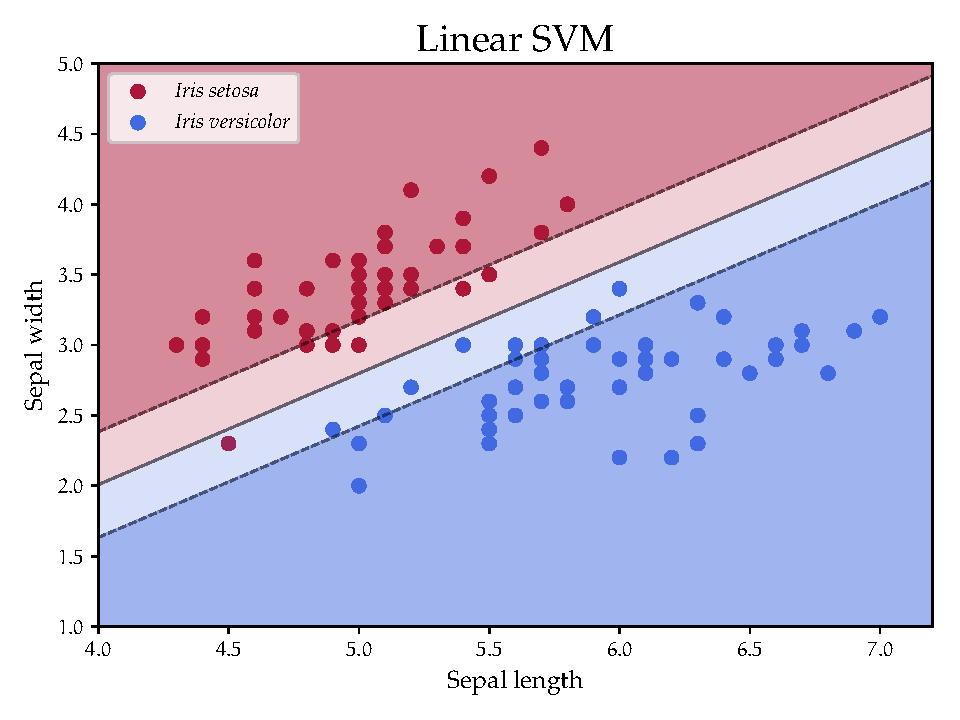
\includegraphics[width=0.45\textwidth]{machine_learning/figures/svm.pdf}}%
\hfill
\subcaptionbox{RBF kernel\label{subfig:svm_rbf}}{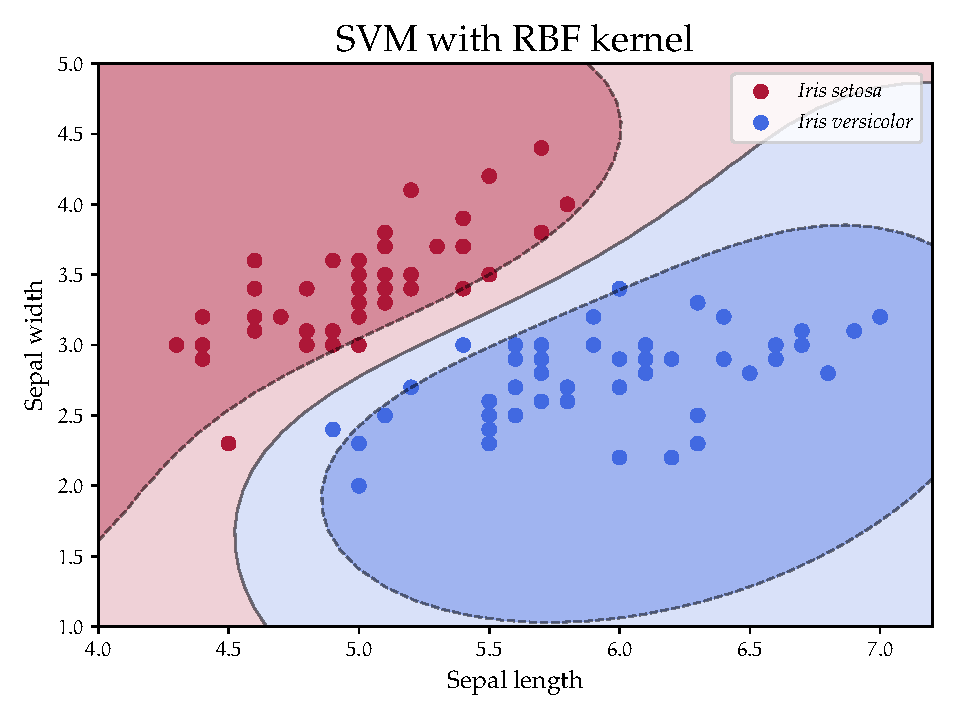
\includegraphics[width=0.45\textwidth]{machine_learning/figures/svm_rbf.pdf}}%
\caption{Classification of two species of Iris flowers according to the length and width of sepals.}\label{fig:svm}
\end{figure}

It can be generalised \marginpar{The kernel trick} to non-flat boundaries using the so-called \emph{kernel trick}, where Euclidean distances are replaced with an arbitrary measure of similarity given by positive-definite kernel function:
\[||\vec{x}_1 - \vec{x}_2|| \rightarrow k(\vec{x}_1, \vec{x}_2)\]

For example, in Figure~\ref{subfig:svm_rbf} we have used a Radial Basis Function:

\[k(\vec{x}_1, \vec{x}_2) = e^{-\gamma ||\vec{x}_1 - \vec{x}_2||^2 },\]
which implicitly projects the data into an infinite-dimensional space.

Another way of interpreting the kernel trick is to think of it as learning a deformation of the space that makes the data separable by a hyperplane, a linear function.

\subsection{$k$-Nearest Neighbour}
A Nearest Neighbour classifier takes the $k$ closest points in the training set, and predicts the most common label.
\marginpar{Bias-variance tradeoff}
The choice of $k$ is a balance between noise and flexibility: smaller values give more distinct frontiers, but are more susceptible to noise.

\begin{figure}[htb]
	\centering
	\subcaptionbox{Closest neighbour}{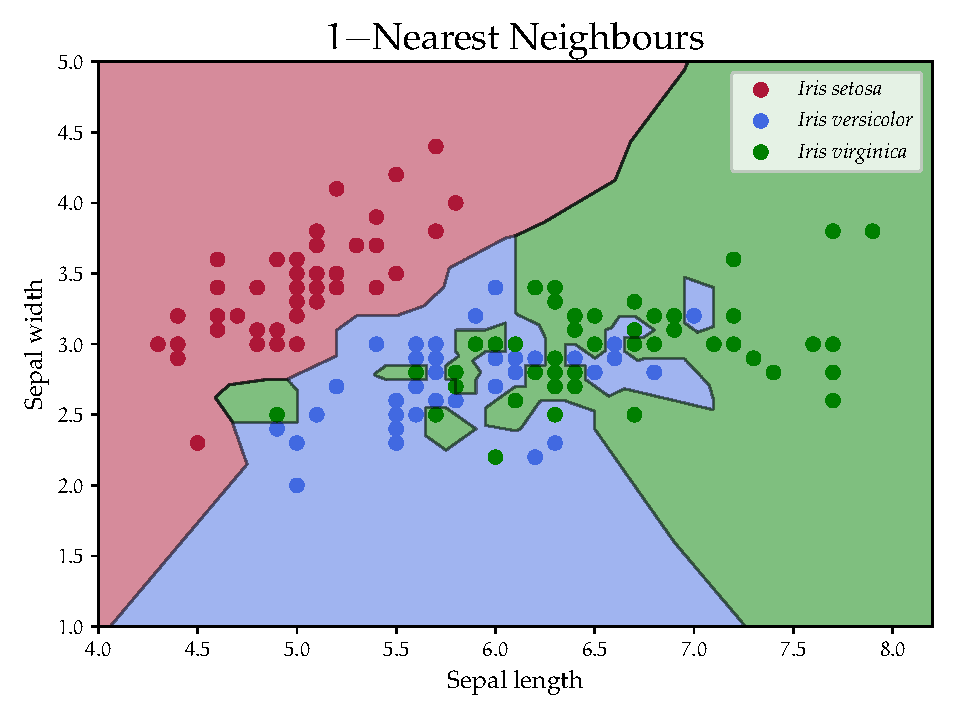
\includegraphics[width=0.45\textwidth]{machine_learning/figures/knn_1}}
	\hfill
	\subcaptionbox{Average of the five closest neighbours.}{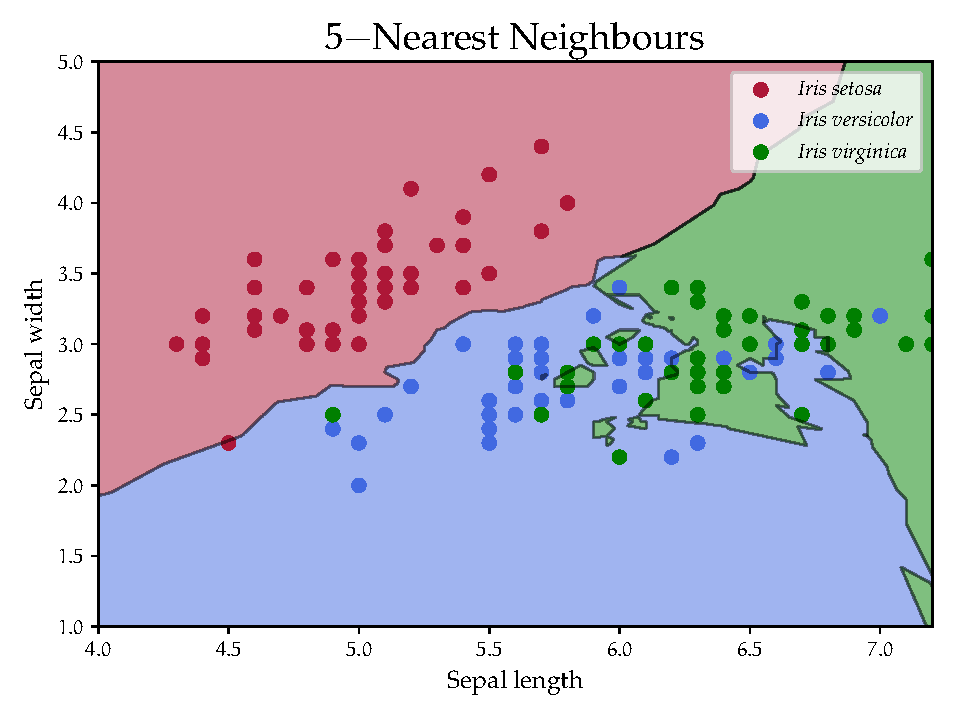
\includegraphics[width=0.45\textwidth]{machine_learning/figures/knn_5}}
	\caption{Classification of three species of Iris flowers according to the length and width of sepals.}\label{fig:knn}
\end{figure}

\subsection{Decision tree}\label{sec:decision_tree}
Decision trees are based on a measure of impurity of a sample: the more homogeneous, the less impure it is.
The most common is the Gini impurity:

\[ G(\vec x) = \sum_k p_{k} (1-p_k),\]
where $p_k$ is the fraction of labels equal to $k$ in the group.

A decision tree splits recursively the training based on the feature that gives the highest decrease in Gini impurity, as illustrated on the Figure~\ref{subfig:gini}.
The final result is a series of simple boolean rules that can be interpreted by humans.
Figure~\ref{subfig:tree_explained} is an example: the root of the tree (shown in white) contains all the training points, and each branch splits it according to a single feature.
The process is repeated until no more cuts can improve the performance, or until the tree reaches a maximum depth.


\begin{figure}[htb]
	\centering
	\subcaptionbox{The rules of a decision tree are interpretable. The shading corresponds to the purity of the node.\label{subfig:tree_explained}}{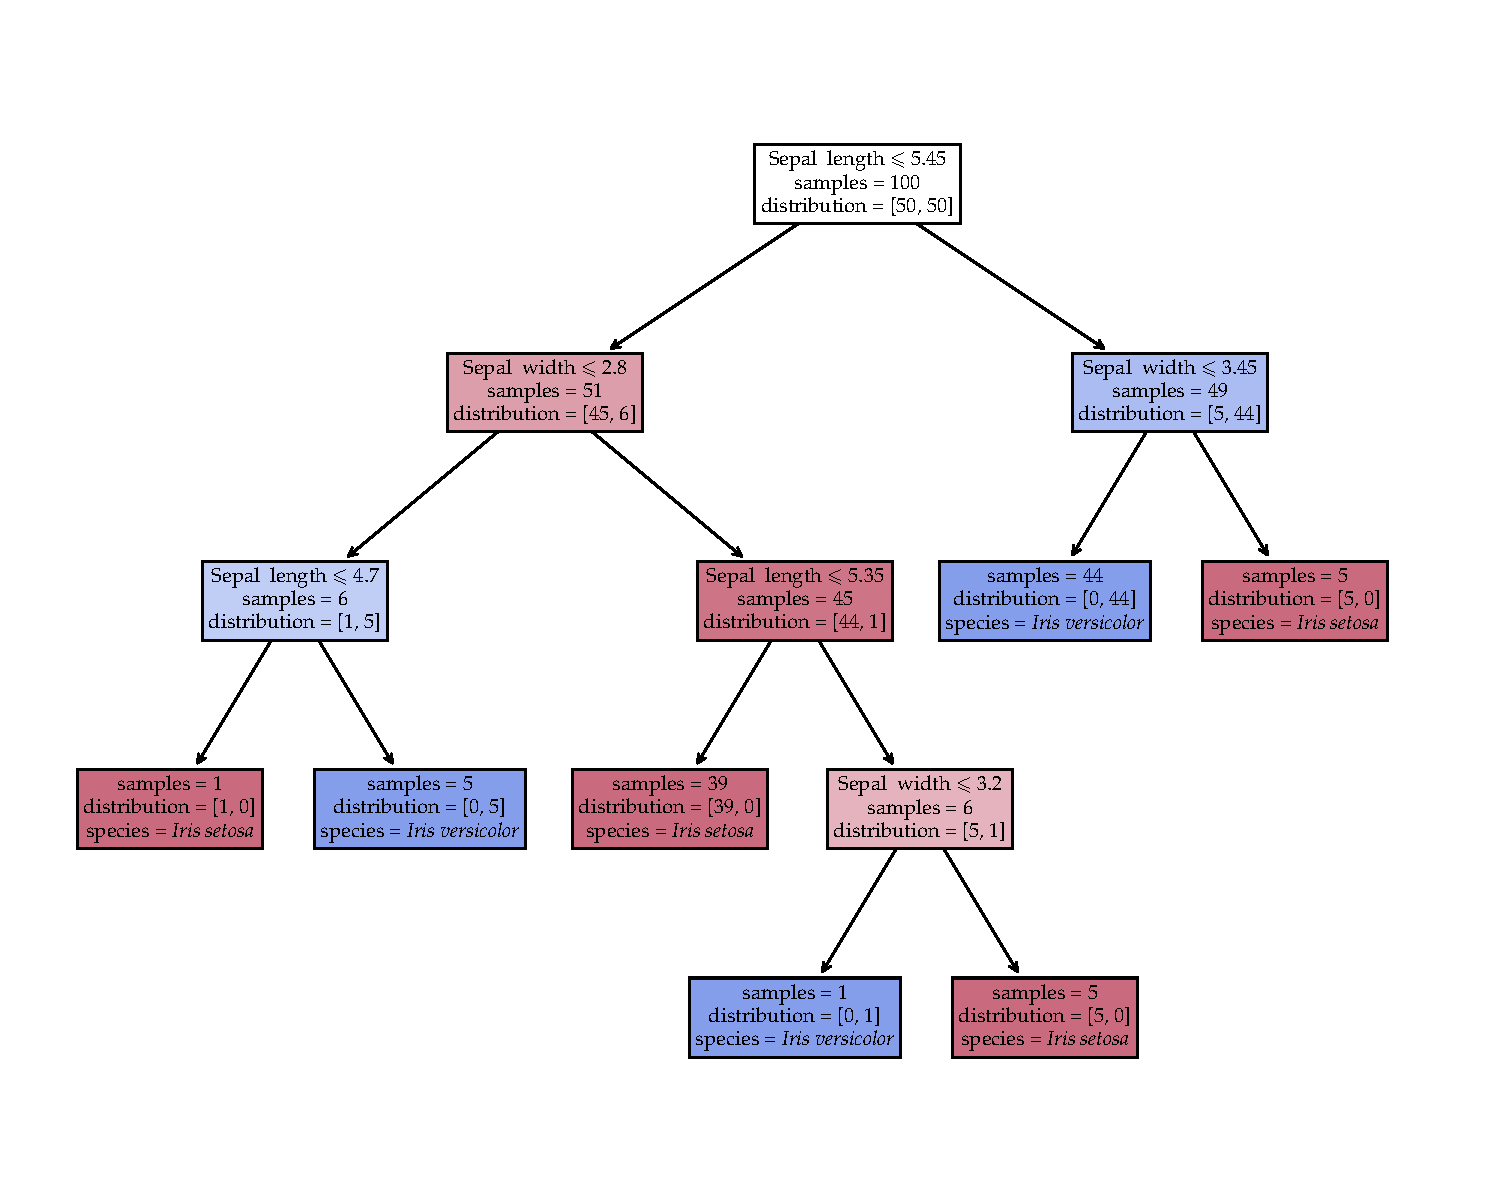
\includegraphics[width=\textwidth]{machine_learning/figures/tree}}
	\\
	\subcaptionbox{Gini impurity as a function of the first split. The ideal cut is selected.\label{subfig:gini}}{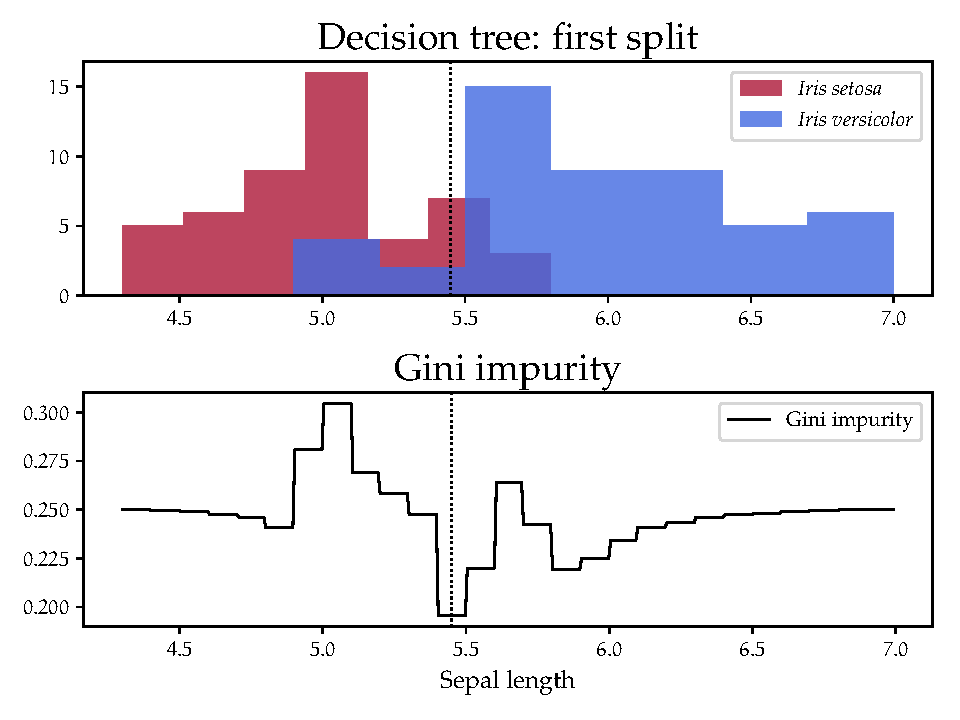
\includegraphics[width=0.45\textwidth]{machine_learning/figures/tree_split}}
	\hfill
	\subcaptionbox{Regions predicted by the tree.\label{subfig:tree}}{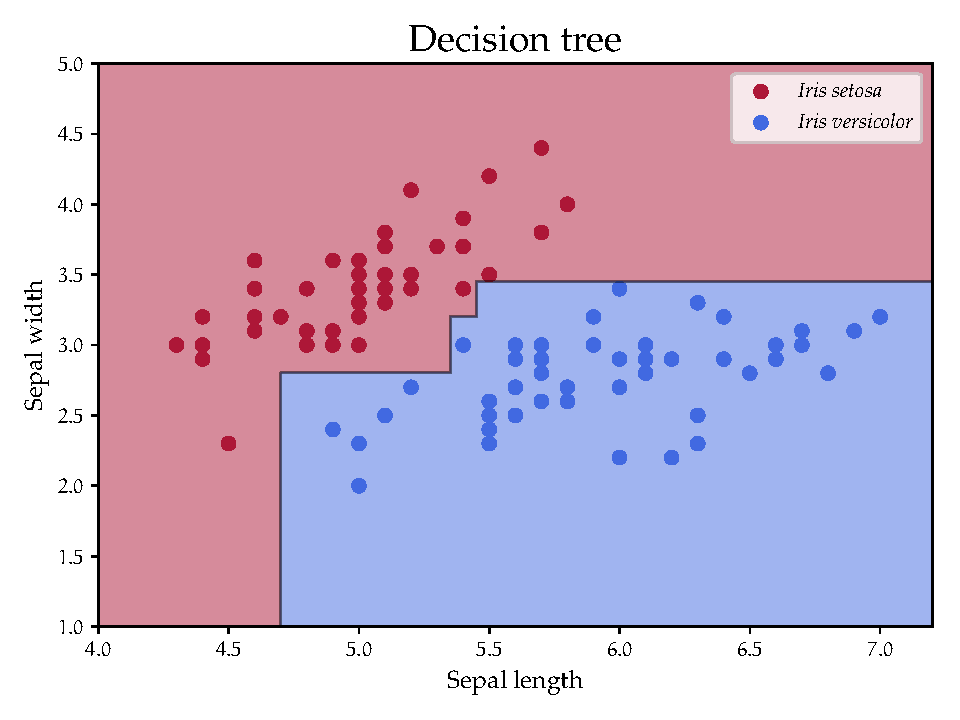
\includegraphics[width=0.45\textwidth]{machine_learning/figures/tree_2d}}
	\caption{Predictions made by a decision tree on the Iris dataset. }\label{fig:tree}
\end{figure}


\subsection{Random Forest}\label{sec:random_forest}
A Random Forest is an ensemble of decision trees, as described in the section~\ref{sec:decision_tree}.
Each tree is trained on a random subset of the data, and the final score is a vote across the trees.
Furthermore, for every split, we only consider a new random subset of the features, to increase diversity.
The advantage over a single decision tree is that now we have an ensemble of trees, each trained on slightly different data.
\marginpar{Bias-variance tradeoff}
Since every data point is only considered by a fraction of the trees, the random forest is more robust against noise; but for the same reason, it will not be able to model so well outliers.


\subsection{Gaussian Processes}
A Gaussian Process (GP) takes as an input a set of data points $(x, y)$ that are assumed to be generated by a latent, unknown function $f(x)$ that we wish to infer, plus Gaussian noise. The output is a \emph{probability distribution} over functions, that should be interpreted as the likelihood for each given function to have produced the observed data.


\begin{figure}[htb]
	\centering
	\subcaptionbox{Complete data}{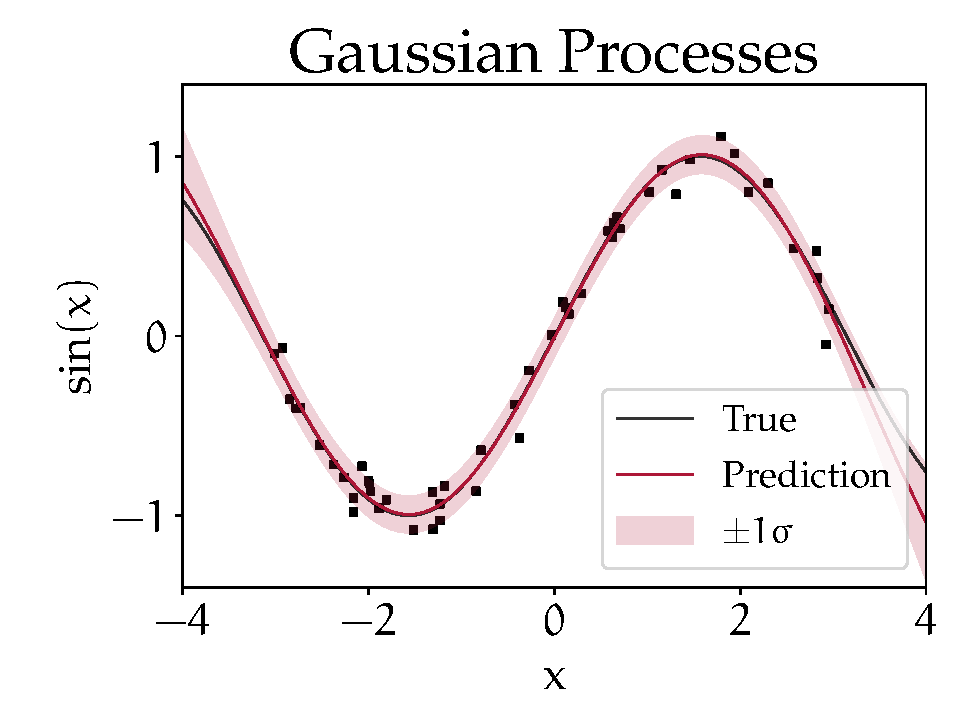
\includegraphics[width=0.45\textwidth]{machine_learning/figures/sin_toy}}
	\hfill
	\subcaptionbox{Gapped data.}{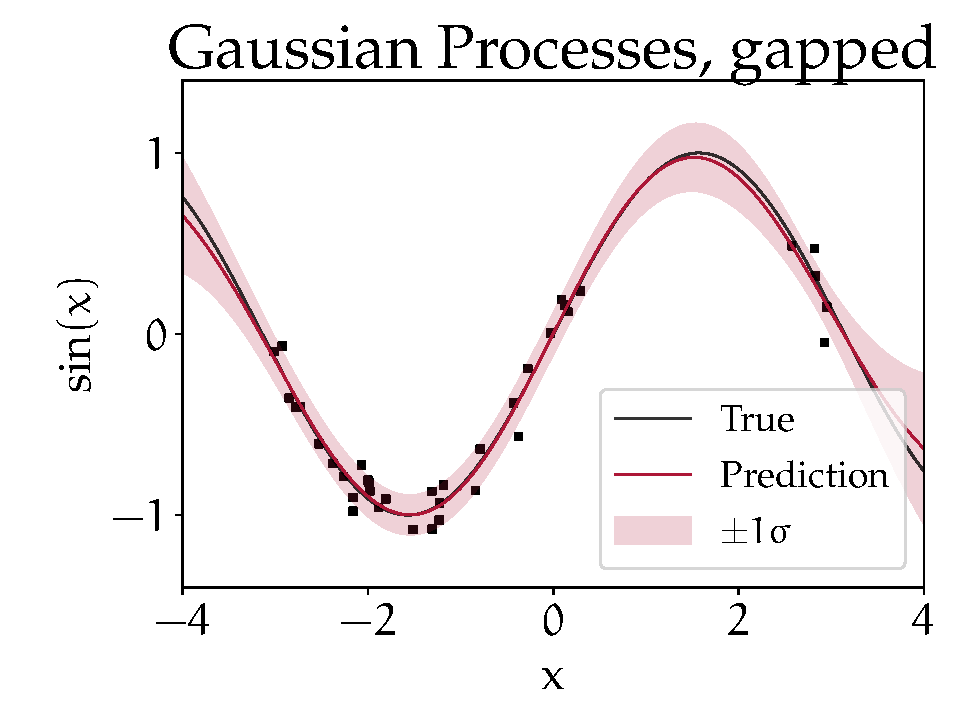
\includegraphics[width=0.45\textwidth]{machine_learning/figures/sin_toy_gapped}}
	\caption{Reconstruction of the $\sin$ function using Gaussian Processes.
	Note the larger uncertainty when there is a gap in the training set.}\label{fig:gp_toy}
\end{figure}


Consider a vector space over functions\footnote{This is a mathematical justification. If you are not interested in Hilbert spaces, jump to the last equation.}, called Hilbert space $\mathscr{H}$, and define a complete, orthonormal basis $\{\phi_i(x)\}_{i=0}^{n}$.
Any function $f$ in this space can be decomposed as a linear combination of the basis:

 \[f(x) = \sum_{i=0}^{n} c_i \phi_i(x)\]
 
In GP, we define our Hilbert space through a positive semi-definite \emph{covariance function} $k(x, x')$.
This induces a metric defined through the distance:

	\[	d(f, g) =\int_{\mathcal{R}}  f(x) k(x, x') g(x') dx dx', \]
and a series of eigenfunctions of the covariance function.
	
For example,\marginpar{RBF appears again} the previously seen radial basis covariance function defines the Hilbert space of $C^\infty \cap L^2$ functions: all the smooth functions of squared-integrable..
	
The GP will thus project our $n$ data points into this $N$ dimensional space (in general, $N >> n$; usually $N = \infty$). Note that, due to geometry, our $n$ data points must live in a $n$-dimensional subspace of $\mathscr{H}$.
The output is an estimation $\hat f$ of our latent function $f$, that can be interpreted as a decomposition in the eigenfunctions of our covariance function.
	
	\[\hat f(x) = \sum_{i=0}^{n} c_i \phi_i(x)\]
	
But, unlike other procedures, $c_i$ have probability distributions over them.
We can use them to sample likely candidates for the latent function, as shown in the Figure~\ref{fig:gp_sampling}
	
\begin{figure}[hbt]
\centering
	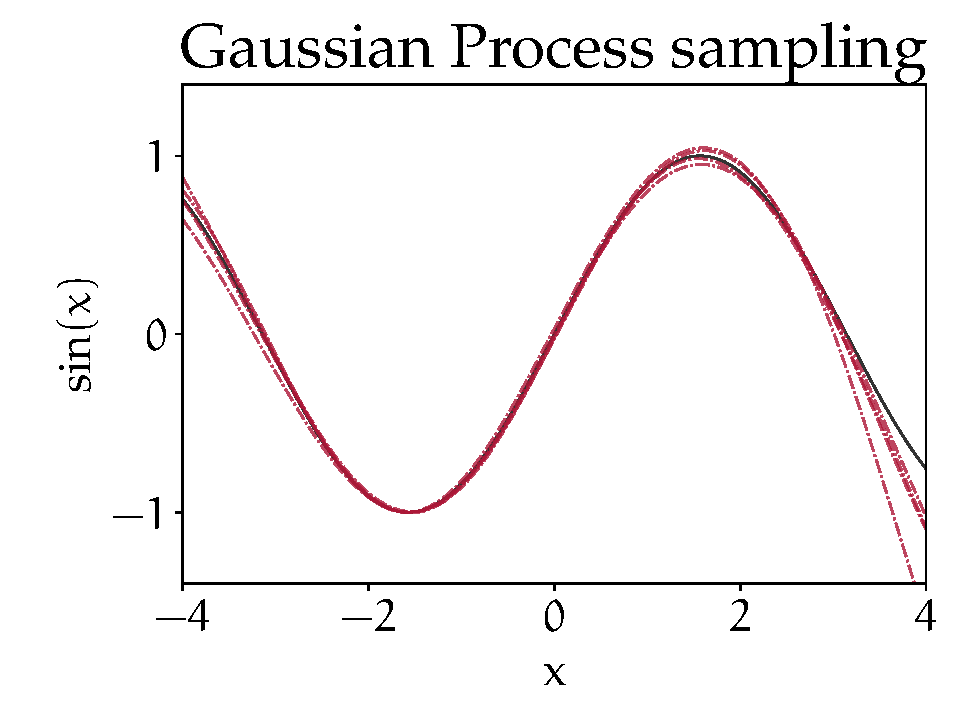
\includegraphics[width=0.45\textwidth]{machine_learning/figures/sin_samples}
	\caption{Posterior samples from Gaussian Processes.}\label{fig:gp_sampling}
\end{figure}

\subsection{Isotonic regression}
Isotonic regression minimises the squared errors of a function that is piecewise constant, and non decreasing.
Given enough data points, it can fit arbitrarily complex curves, as long as they are monotonous.
This method is particularly useful in calibration to turn predicted scores into actual probabilities.
\todo{figure}

\section{On the wrongness of machine learning}\label{sec:wrong}
The results of machine learning can be 
\todo[inline]{TODO}
